% =====================================================================
\chapter{Modulo 6 -- Complessità Computazionale}
% =====================================================================

% ---------------------------------------------------------------------
\section{Teoria \& Analogia Chiave}
% ---------------------------------------------------------------------

\begin{consiglio}[: come affrontare questo modulo]
Il modulo lavora su due piani, e servono entrambi. Il primo è \textbf{pratico}:
contare quante volte il computer ripete un'operazione quando i dati crescono, e
riconoscere a colpo d'occhio la complessità di un ciclo. Tutti i programmi del modulo
\emph{contano davvero} i passi con un contatore e stampano i risultati, così ogni
formula si può verificare con i numeri. Il secondo è \textbf{formale}: le definizioni
di $O$, $\Omega$ e $\Theta$ con le costanti $c$ e $n_0$, le loro proprietà e la
soluzione delle ricorrenze. Al quiz e all'orale vengono chieste entrambe le cose:
leggi la teoria con carta e penna e rifai da solo ogni dimostrazione.
\end{consiglio}

\subsection*{Perché misurare un algoritmo}

Due programmi risolvono lo stesso problema. Su 10 dati impiegano entrambi un
istante. Su un milione di dati uno finisce in un secondo, l'altro in tre giorni.
Questa differenza non dipende dal computer: dipende da \textbf{come cresce il
lavoro} quando crescono i dati. È questo che misura la \textbf{complessità
computazionale}.

Non si misura in secondi, perché i secondi dipendono dalla macchina, dal
compilatore e da cosa sta facendo il PC in quel momento. Si misura in
\textbf{numero di operazioni elementari} (\textbf{passi}): un'assegnazione, un
confronto, una somma, l'accesso a \cc|v[i]|. Questa è la prima \textbf{ipotesi
semplificativa} delle slide: \emph{ogni operazione elementare costa 1}, e il
tempo è proporzionale al numero di operazioni. È il cosiddetto \textbf{modello RAM}.

Il numero di passi dipende dalla \textbf{dimensione dell'input}, che si indica con
$n$: quanti elementi ha l'array, quanti nodi ha la lista, quante cifre ha il
numero. La complessità in tempo è quindi una funzione $T : \mathbb{N} \to \mathbb{N}$
che a ogni dimensione $n$ associa il numero di passi.

Si parla di complessità in \textbf{tempo} (quanti passi) e in \textbf{spazio}
(quante celle di memoria \emph{in più} servono, oltre a quelle che contengono
l'input; per una funzione ricorsiva vanno contati anche i record di attivazione
presenti contemporaneamente sullo stack).

\subsection*{Le regole per contare}

Le slide del corso danno queste regole di composizione:
\begin{itemize}
  \item \textbf{Sequenza} di istruzioni: si \textbf{sommano} i costi,
        $T_{A;B}(n) = T_A(n) + T_B(n)$.
  \item \textbf{if-else}: costo della condizione più il \textbf{maggiore} tra i
        due rami. Non sapendo quale ramo verrà eseguito, ci si mette nel caso più
        costoso.
  \item \textbf{Ciclo} (\cc|for|, \cc|while|, \cc|do-while|): si sommano i costi di
        \textbf{tutti i giri} (corpo più condizione). Se il corpo costa sempre uguale,
        è \emph{numero di giri $\times$ costo di un giro}; se il costo dipende
        dall'indice, si ottiene una \textbf{sommatoria} (vedi più avanti).
  \item \textbf{Chiamata di funzione}: costa quanto il suo corpo (più il passaggio
        dei parametri). Per le funzioni ricorsive il costo si scrive con una
        \textbf{relazione di ricorrenza}.
\end{itemize}

\subsection*{Caso migliore, peggiore e medio}

Lo stesso algoritmo, con la stessa $n$, può fare un numero di passi diverso a
seconda dei dati. Cercare un nome in un elenco di 1000 nomi controllandoli uno a uno:
se è il primo basta 1 confronto, se è l'ultimo (o non c'è) ne servono 1000.
Formalmente, se $I_n$ è l'insieme degli input di dimensione $n$ e $t(x)$ i passi
sull'input $x$:
\begin{itemize}
  \item \textbf{caso migliore}: $T_{\min}(n) = \min_{x \in I_n} t(x)$ (1 confronto);
  \item \textbf{caso peggiore}: $T_{\max}(n) = \max_{x \in I_n} t(x)$ (1000 confronti);
  \item \textbf{caso medio}: $T_{\text{med}}(n) = \sum_{x \in I_n} P(x)\, t(x)$, la media
        pesata con la probabilità di ogni input. Per la ricerca sequenziale con
        l'elemento presente e posizioni equiprobabili:
        $\frac{1}{n}\sum_{i=1}^{n} i = \frac{n+1}{2}$, circa 500.
\end{itemize}
Salvo indicazione diversa, \textbf{si studia il caso peggiore}: è una
\emph{garanzia}, perché l'algoritmo non farà mai peggio di così, e a differenza del
caso medio non richiede ipotesi sulla distribuzione degli input.
L'Esercizio~6.5 misura i tre casi.

\subsection*{Conta solo la crescita: la seconda ipotesi semplificativa}

Trovare la formula \emph{esatta} dei passi è spesso difficile, e soprattutto poco
utile. Guarda questa tabella (Esercizio~6.4): un programma esegue prima un ciclo
da $n$ giri, poi due cicli annidati da $n \times n$ giri.

\begin{center}
\begin{tabular}{rrrr}
\toprule
$n$ & primo blocco ($n$) & secondo blocco ($n^2$) & quota del secondo \\
\midrule
10   & 10    & 100        & 91\% \\
100  & 100   & 10\,000    & 99\% \\
1000 & 1000  & 1\,000\,000 & 99,9\% \\
\bottomrule
\end{tabular}
\end{center}
Quando $n$ è grande il primo blocco è trascurabile: il tempo lo decide il blocco più
pesante. Lo stesso vale per le costanti moltiplicative: un ciclo che fa $n/2$ giri o
$3n$ giri cresce \emph{come} $n$, e le costanti dipendono comunque dalla macchina e
dal compilatore. Ci interessa quindi l'\textbf{ordine di crescita} di $T(n)$ per
$n \to \infty$: il \textbf{comportamento asintotico}. Le notazioni che seguono servono
a dirlo in modo preciso.

\subsection*{La notazione O-grande}

\begin{definizione}[: O-grande]
Date due funzioni $f, g : \mathbb{N} \to \mathbb{R}^{+}$,
\[
f(n) = O(g(n)) \iff \exists\, c > 0,\ \exists\, n_0 \in \mathbb{N} \ \text{tali che}\
f(n) \le c \cdot g(n) \quad \forall\, n \ge n_0 .
\]
Si legge \q{$f$ è o grande di $g$}: \textbf{$f$ non cresce più in fretta di $g$}.
\end{definizione}

Leggiamo la definizione pezzo per pezzo:
\begin{itemize}
  \item \q{esiste $c$}: si può moltiplicare $g$ per una costante scelta a piacere.
        È questo che rende irrilevanti le costanti moltiplicative.
  \item \q{esiste $n_0$}: per i primi valori di $n$ può succedere di tutto; conta solo
        il comportamento \q{da $n_0$ in poi}.
  \item \q{$f(n) \le c\, g(n)$}: da quel punto in avanti, il grafico di $f$ resta sotto
        quello di $c\,g$ (il disegno è nella sezione successiva).
\end{itemize}
Formalmente $O(g(n))$ è un \emph{insieme} di funzioni, e $f = O(g)$ è un abuso di
notazione per $f \in O(g)$: per questo l'uguaglianza non è simmetrica
($n = O(n^2)$ è vero, $n^2 = O(n)$ è falso).

\textbf{Dimostrare che $f = O(g)$} significa \textbf{esibire} una coppia $(c, n_0)$
che funziona. Due esempi delle slide:
\begin{itemize}
  \item $8n - 2 = O(n)$: per ogni $n \ge 1$ vale $8n - 2 \le 8n$, quindi bastano
        $c = 8$ e $n_0 = 1$.
  \item $5n^4 + 3n^3 + 2n^2 + 4n + 7 = O(n^4)$: per $n \ge 1$ ogni potenza $n^k$ con
        $k \le 4$ è al più $n^4$ (e $7 \le 7n^4$), quindi
        $5n^4 + 3n^3 + 2n^2 + 4n + 7 \le (5+3+2+4+7)\, n^4 = 21\, n^4$.
        Bastano $c = 21$ e $n_0 = 1$.
\end{itemize}
Le coppie valide sono infinite: con $c$ più grande si può spesso scegliere $n_0$ più
piccolo, e viceversa. Ne basta una.

\textbf{Dimostrare che $f \neq O(g)$} significa mostrare che \emph{nessuna} coppia
funziona; di solito si ragiona per assurdo. Esempio: $n^2 \neq O(n)$. Se esistessero
$c$ e $n_0$ con $n^2 \le c\,n$ per ogni $n \ge n_0$, dividendo per $n > 0$ si
avrebbe $n \le c$ per ogni $n \ge n_0$: falso, perché basta prendere
$n = \max(n_0, \lceil c \rceil + 1)$.

\textbf{Attenzione a un dettaglio da quiz.} O-grande è \textbf{un} limite superiore,
non \textbf{il} limite superiore. Se un algoritmo è $O(n^2)$ è anche $O(n^3)$ e
$O(2^n)$. Si indica, ovviamente, il limite più stretto, cioè il più informativo.

\subsection*{Le sorelle: Omega e Theta}

\begin{definizione}[: Omega-grande e Theta-grande]
\[
f(n) = \Omega(g(n)) \iff \exists\, c > 0,\ \exists\, n_0 \ \text{tali che}\
f(n) \ge c \cdot g(n) \quad \forall\, n \ge n_0
\]
\[
f(n) = \Theta(g(n)) \iff \exists\, c_1, c_2 > 0,\ \exists\, n_0 \ \text{tali che}\
c_1\, g(n) \le f(n) \le c_2\, g(n) \quad \forall\, n \ge n_0
\]
\end{definizione}

\begin{center}
\begin{tabular}{lll}
\toprule
\textbf{Notazione} & \textbf{A parole} & \textbf{Ruolo} \\
\midrule
$f = O(g)$      & $f$ cresce \textbf{al più} come $g$  & limite superiore (\q{non peggio di}) \\
$f = \Omega(g)$ & $f$ cresce \textbf{almeno} come $g$  & limite inferiore (\q{non meglio di}) \\
$f = \Theta(g)$ & $f$ cresce \textbf{esattamente} come $g$ & limite stretto: $O(g)$ e $\Omega(g)$ \\
\bottomrule
\end{tabular}
\end{center}
($\Omega$ si legge \q{omega grande}, $\Theta$ \q{theta grande}.) Dalle definizioni
seguono subito due fatti:
\[
f = \Theta(g) \iff f = O(g) \ \text{e}\ f = \Omega(g), \qquad\qquad
f = O(g) \iff g = \Omega(f).
\]
Il secondo (\textbf{dualità}) si dimostra dividendo per $c$: se $f \le c\,g$ allora
$g \ge \frac{1}{c} f$.

\textbf{Esempio completo.} Dimostriamo che $T(n) = 3n^2 + 5n + 7 = \Theta(n^2)$.
\begin{itemize}
  \item \emph{Limite superiore.} Per $n \ge 1$: $5n \le 5n^2$ e $7 \le 7n^2$, quindi
        $T(n) \le 3n^2 + 5n^2 + 7n^2 = 15\,n^2$. Scegliamo $c_2 = 15$.
  \item \emph{Limite inferiore.} I termini $5n$ e $7$ sono positivi, quindi
        $T(n) \ge 3n^2$ per ogni $n$. Scegliamo $c_1 = 3$.
  \item Con $n_0 = 1$ vale $3n^2 \le T(n) \le 15n^2$ per ogni $n \ge n_0$. $\square$
\end{itemize}
Lo stesso ragionamento dimostra il risultato generale: \textbf{un polinomio di grado
$k$ con coefficiente direttore positivo è $\Theta(n^k)$}. Per l'Omega si sceglie
$c_1 = a_k/2$: i termini di grado minore, divisi per $n^k$, tendono a zero e da un
certo $n_0$ in poi in valore assoluto sono minori di $a_k/2$.

\textbf{Le versioni strette.} Esistono anche $o$-piccolo e $\omega$-piccolo:
$f = o(g)$ se per \emph{ogni} $c > 0$ esiste $n_0$ con $f(n) < c\,g(n)$ da $n_0$ in
poi, cioè $f$ cresce \emph{strettamente} meno di $g$ (per esempio $n = o(n^2)$, ma
$n^2 \neq o(n^2)$). $\omega$ è il duale.

\subsection*{Il criterio del limite}

Quando le funzioni sono \q{regolari}, il modo più rapido per confrontarle è il limite
del rapporto. Se esiste
\[
L = \lim_{n \to \infty} \frac{f(n)}{g(n)}
\]
allora:
\begin{center}
\begin{tabular}{ll}
\toprule
\textbf{Valore di $L$} & \textbf{Conclusione} \\
\midrule
$0 < L < \infty$ & $f = \Theta(g)$ \\
$L = 0$ & $f = O(g)$ ma $f \neq \Theta(g)$ (anzi $f = o(g)$) \\
$L = \infty$ & $f = \Omega(g)$ ma $f \neq \Theta(g)$ (anzi $f = \omega(g)$) \\
\bottomrule
\end{tabular}
\end{center}
Perché funziona: se il rapporto tende a $L$ finito, da un certo $n_0$ in poi è
compreso, per esempio, tra $L/2$ e $2L$, che sono proprio le costanti $c_1$ e $c_2$
della definizione di $\Theta$. Il criterio non si applica se il limite non esiste
(per esempio con funzioni che oscillano): in quel caso si torna alla definizione.

Esempi che conviene saper rifare:
\begin{itemize}
  \item $\lim \frac{\log n}{n} = 0$ (con de l'Hôpital: $\frac{1/(n \ln 2)}{1} \to 0$),
        quindi $\log n = o(n)$. Più in generale $\log^k n = o(n^\varepsilon)$ per ogni
        $k$ e ogni $\varepsilon > 0$: \textbf{qualunque potenza del logaritmo cresce meno
        di qualunque potenza di $n$}.
  \item $\lim \frac{n^k}{2^n} = 0$ per ogni $k$ (de l'Hôpital applicato $k$ volte):
        \textbf{ogni polinomio cresce meno di ogni esponenziale}.
  \item $\lim \frac{3n^2 + 5n + 7}{n^2} = 3$: ritroviamo $\Theta(n^2)$.
\end{itemize}

\subsection*{Proprietà da usare senza ridimostrarle}

Per ogni $f, g, h$ positive e costante $a > 0$:
\begin{itemize}
  \item \textbf{Costanti}: $a \cdot f = \Theta(f)$.
  \item \textbf{Somma (regola del massimo)}: $f + g = \Theta(\max(f, g))$. Infatti
        $\max(f,g) \le f + g \le 2 \max(f, g)$. È la regola dei blocchi in sequenza:
        conta il più pesante.
  \item \textbf{Prodotto}: se $f_1 = O(g_1)$ e $f_2 = O(g_2)$ allora
        $f_1 f_2 = O(g_1 g_2)$ (si moltiplicano le costanti). È la regola dei cicli
        annidati.
  \item \textbf{Transitività}: $f = O(g)$ e $g = O(h)$ implicano $f = O(h)$ (con
        costante $c_1 c_2$ e soglia $\max(n_1, n_2)$); vale anche per $\Omega$ e
        $\Theta$.
  \item \textbf{Riflessività e simmetria}: $f = \Theta(f)$; $f = \Theta(g) \iff g = \Theta(f)$.
        $\Theta$ è quindi una relazione di equivalenza: le sue classi sono le
        \textbf{classi di complessità}.
\end{itemize}

\textbf{La base del logaritmo non conta.} Per il cambio di base
$\log_a n = \frac{\log_b n}{\log_b a}$, e $\frac{1}{\log_b a}$ è una costante: quindi
$\log_a n = \Theta(\log_b n)$ per ogni $a, b > 1$, e si scrive semplicemente
$O(\log n)$. Ricorda anche $\log(n^k) = k \log n = \Theta(\log n)$. Attenzione invece
agli esponenziali: $3^n \neq O(2^n)$, perché $3^n/2^n = (3/2)^n \to \infty$.

\subsection*{Le classi di complessità da conoscere}

Questa è la tabella più importante del modulo: i numeri sono i passi \emph{veri}
contati dal pattern di codice ($\log$ in base 2).

\begin{center}\small
\begin{tabular}{llrrl}
\toprule
\textbf{Classe} & \textbf{Nome} & $n = 1000$ & $n = 10\,000$ & \textbf{Esempio} \\
\midrule
$O(1)$        & costante     & 1          & 1           & accesso a \texttt{v[i]} \\
$O(\log n)$   & logaritmica  & 10         & 14          & ricerca binaria \\
$O(n)$        & lineare      & 1000       & 10\,000     & ricerca sequenziale \\
$O(n \log n)$ & pseudolineare & 10\,000 & 140\,000  & MergeSort \\
$O(n^2)$      & quadratica   & 1\,000\,000 & 100\,000\,000 & Bubble, Selection, Insertion \\
$O(2^n)$      & esponenziale & \multicolumn{2}{c}{numeri astronomici} & tutti i sottoinsiemi \\
\bottomrule
\end{tabular}
\end{center}

La gerarchia, dimostrabile con il criterio del limite, è
\[
1 \;<\; \log n \;<\; \sqrt{n} \;<\; n \;<\; n \log n \;<\; n^2 \;<\; n^3 \;<\; 2^n \;<\; n! \;<\; n^n
\]
dove $f < g$ significa $f = o(g)$. Come leggerla in pratica:
\begin{itemize}
  \item $O(1)$: il lavoro non dipende da $n$.
  \item $O(\log n)$: ogni passo elimina una frazione costante del problema (di
        solito metà). Moltiplicando i dati per 10 si aggiungono solo 3--4 passi; con un
        milione di dati, 20 passi.
  \item $O(n)$: dati doppi, lavoro doppio.
  \item $O(n \log n)$: poco più che lineare. È il prezzo ottimo dell'ordinamento per
        confronti (Modulo 7).
  \item $O(n^2)$: dati $\times 10$, lavoro $\times 100$. Con un milione di dati sono
        mille miliardi di passi.
  \item $O(2^n)$: ogni elemento in più \emph{raddoppia} il lavoro; inutilizzabile già
        con poche decine di dati (Esercizio~6.10).
\end{itemize}

\begin{analogia}[: la rubrica telefonica]
Devi trovare \q{Rossi} in una rubrica di 1000 pagine. Metodo 1: sfogli dalla prima
pagina finché non lo trovi; nel caso peggiore 1000 pagine, $O(n)$. Metodo 2: apri a
metà, vedi che sei alla \q{M}, quindi Rossi è nella seconda metà; scarti la prima
metà e riapri a metà di quello che resta. Dopo $k$ aperture restano $n/2^k$ pagine,
e ci si ferma quando $n/2^k = 1$, cioè $k = \log_2 n$: circa 10 aperture,
$O(\log n)$. Con una rubrica di un milione di pagine il primo metodo ne guarda un
milione, il secondo una ventina. Il logaritmo in base 2 di $n$ è proprio questo:
\textbf{quante volte si può dimezzare $n$ prima di arrivare a 1}.
\end{analogia}

\subsection*{Riconoscere la complessità a colpo d'occhio}

Nella maggior parte dei casi basta guardare \textbf{come si muovono i cicli}:
\begin{center}
\begin{tabular}{p{7.2cm}l}
\toprule
\textbf{Struttura} & \textbf{Complessità} \\
\midrule
istruzioni senza cicli né chiamate & $O(1)$ \\
un ciclo con \cc|i += c| o \cc|i -= c| fino a $n$ (c costante) & $O(n)$ \\
un ciclo con \cc|i *= c| o \cc|i /= c| (c costante $>1$) & $O(\log n)$ \\
due cicli \textbf{annidati}, ognuno $O(n)$ (anche \q{a triangolo}) & $O(n^2)$ \\
tre cicli annidati $O(n)$ & $O(n^3)$ \\
cicli annidati di tipo diverso & \textbf{prodotto} delle complessità \\
blocchi \textbf{in sequenza} & quello \textbf{più pesante} \\
\bottomrule
\end{tabular}
\end{center}

Esempio delle slide (Esercizio~6.6):
\begin{lstlisting}
for (i = n/2; i <= n; i++)          // circa n/2 giri         -> O(n)
    for (j = 1; j <= n; j = 2*j)    // raddoppia              -> O(log n)
        for (k = 1; k <= n; k = k*2)//  raddoppia             -> O(log n)
            count++;                // totale: O(n * log n * log n)
\end{lstlisting}

\textbf{Le sommatorie da conoscere.} Quando il numero di giri del ciclo interno dipende
dall'indice esterno, il costo è una somma:
\begin{itemize}
  \item \textbf{Serie aritmetica} (somma di Gauss): $\displaystyle\sum_{i=1}^{n} i = \frac{n(n+1)}{2} = \Theta(n^2)$.
        Il ciclo \q{a triangolo} \cc|for (j = i + 1; j < n; j++)| fa
        $(n-1) + (n-2) + \cdots + 1 = \frac{n(n-1)}{2}$ giri: metà del quadrato
        pieno, ma sempre $\Theta(n^2)$. In generale $\sum_{i=1}^{n} i^k = \Theta(n^{k+1})$.
  \item \textbf{Serie geometrica}: $\displaystyle\sum_{i=0}^{k} r^i = \frac{r^{k+1}-1}{r-1}$ per $r \neq 1$.
        Due casi utilissimi: $\sum_{i=0}^{k} 2^i = 2^{k+1} - 1$ (domina l'ultimo
        termine) e $\sum_{i \ge 0} n/2^i \le 2n$ (domina il primo).
  \item \textbf{Somma dei logaritmi}: $\displaystyle\sum_{i=1}^{n} \log i = \log(n!) = \Theta(n \log n)$.
        Dall'alto: ogni termine è al più $\log n$. Dal basso: gli ultimi $n/2$
        termini valgono almeno $\log(n/2)$ ciascuno, quindi la somma è almeno
        $\frac{n}{2}\log\frac{n}{2}$.
\end{itemize}

\subsection*{Complessità di un problema e algoritmi ottimi}

Fin qui abbiamo misurato un \emph{algoritmo}. Si può parlare anche della complessità
di un \emph{problema}:
\begin{itemize}
  \item un algoritmo che lo risolve in $O(f(n))$ dà un \textbf{limite superiore}
        alla complessità del problema;
  \item se si dimostra che \textbf{ogni} algoritmo richiede almeno $f(n)$ passi nel
        caso peggiore, si ha un \textbf{limite inferiore} $\Omega(f(n))$;
  \item quando i due coincidono, l'algoritmo è \textbf{ottimo} e la complessità del
        problema è $\Theta(f(n))$.
\end{itemize}
Esempio da ricordare: \textbf{ordinare $n$ elementi per confronti richiede
$\Omega(n \log n)$ confronti}. Idea della dimostrazione: un algoritmo per confronti si
può rappresentare come un albero binario di decisione, in cui ogni nodo è un confronto
e ogni foglia una permutazione possibile dell'input. Le permutazioni sono $n!$, quindi
servono almeno $n!$ foglie; un albero binario di altezza $h$ ne ha al più $2^h$, da cui
$h \ge \log_2(n!) = \Theta(n \log n)$ (somma dei logaritmi, sopra). L'altezza è il
numero di confronti nel caso peggiore. MergeSort, che è $O(n \log n)$, è quindi ottimo.

\subsection*{Algoritmi ricorsivi e ricorrenze}

Una funzione ricorsiva chiama se stessa su un problema più piccolo. Il suo costo si
scrive con una \textbf{relazione di ricorrenza}: $T(n)$ espresso con $T$ su valori
più piccoli, più un \textbf{caso base} (di solito $T(1) = \Theta(1)$). Le slide
presentano \textbf{cinque ricorrenze fondamentali}:

\begin{center}\small
\begin{tabular}{p{3.1cm}p{6.6cm}l}
\toprule
\textbf{Ricorrenza} & \textbf{Cosa fa il programma} & \textbf{Soluzione} \\
\midrule
$C_N = C_{N-1} + N$   & toglie un elemento alla volta, ma ogni volta scorre tutto l'input & $\Theta(N^2)$ \\
$C_N = C_{N/2} + 1$   & dimezza l'input con lavoro costante (ricerca binaria) & $\Theta(\log N)$ \\
$C_N = C_{N/2} + N$   & dimezza l'input ma prima lo esamina tutto & $\Theta(N)$ \\
$C_N = 2C_{N/2} + N$  & divide in due metà, risolve entrambe, poi scorre tutto (MergeSort) & $\Theta(N \log N)$ \\
$C_N = 2C_{N/2} + 1$  & divide in due metà, risolve entrambe, lavoro costante in più & $\Theta(N)$ \\
\bottomrule
\end{tabular}
\end{center}

\textbf{Metodo dell'iterazione (srotolamento).} Si sostituisce la ricorrenza in se
stessa finché non si vede lo schema, poi si arriva al caso base. Supponiamo
$N = 2^k$ (cioè $k = \log_2 N$) e $C_1 = 1$ (per la prima, $N$ qualsiasi).
\begin{itemize}
  \item $C_N = C_{N-1} + N = C_{N-2} + (N-1) + N = \cdots = C_1 + 2 + 3 + \cdots + N
        = \frac{N(N+1)}{2}$.
  \item $C_N = C_{N/2} + 1 = C_{N/4} + 2 = \cdots = C_{N/2^k} + k = C_1 + k = \log_2 N + 1$.
  \item $C_N = C_{N/2} + N = C_{N/4} + \frac{N}{2} + N = \cdots
        = C_1 + N\left(1 + \frac12 + \frac14 + \cdots + \frac{2}{N}\right) \le 1 + 2N$
        (serie geometrica di ragione $1/2$).
  \item $C_N = 2C_{N/2} + N$. Dividendo per $N$:
        $\frac{C_N}{N} = \frac{C_{N/2}}{N/2} + 1 = \frac{C_{N/4}}{N/4} + 2 = \cdots
        = \frac{C_1}{1} + k$, quindi $C_N = N(\log_2 N + 1) = \Theta(N \log N)$.
  \item $C_N = 2C_{N/2} + 1 = 4C_{N/4} + 2 + 1 = \cdots = 2^k C_1 + (2^{k-1} + \cdots + 2 + 1)
        = N + (N - 1) = 2N - 1$.
\end{itemize}
Il risultato per $N = 2^k$ si estende a ogni $N$ perché le funzioni coinvolte sono
monotone: tra due potenze di 2 consecutive il costo cambia al più di un fattore
costante.

\textbf{Albero di ricorsione.} Per $C_N = 2C_{N/2} + N$ si disegna un albero: la
radice costa $N$, i suoi due figli $N/2$ ciascuno, i quattro nipoti $N/4$ ciascuno, e
così via. \textbf{Ogni livello costa in totale $N$} e i livelli sono $\log_2 N + 1$:
totale $N \log N$. Il disegno è nella sezione successiva.

\textbf{Teorema dell'esperto (Master Theorem).} Per le ricorrenze di tipo divide et
impera
\[
T(n) = a\, T(n/b) + f(n), \qquad a \ge 1,\ b > 1,
\]
si confronta $f(n)$ con $n^{\log_b a}$ (il numero di foglie dell'albero di ricorsione):
\begin{enumerate}
  \item se $f(n) = O(n^{\log_b a - \varepsilon})$ per qualche $\varepsilon > 0$
        (vincono le foglie): $T(n) = \Theta(n^{\log_b a})$;
  \item se $f(n) = \Theta(n^{\log_b a})$ (ogni livello costa uguale):
        $T(n) = \Theta(n^{\log_b a} \log n)$;
  \item se $f(n) = \Omega(n^{\log_b a + \varepsilon})$ e $a f(n/b) \le c f(n)$ per
        qualche $c < 1$ (vince la radice): $T(n) = \Theta(f(n))$.
\end{enumerate}
Verifica sulle ricorrenze della tabella: ricerca binaria $a = 1, b = 2$,
$n^{\log_2 1} = 1 = \Theta(f)$, caso 2: $\Theta(\log n)$. MergeSort $a = 2, b = 2$,
$n^{\log_2 2} = n = \Theta(f)$, caso 2: $\Theta(n \log n)$. $C_N = C_{N/2} + N$:
$n^0 = 1$ e $f = n$, caso 3: $\Theta(n)$. $C_N = 2C_{N/2} + 1$: $n^1$ contro
$f = 1$, caso 1: $\Theta(n)$. La prima ricorrenza ($C_{N-1}$) non è di questa forma:
si risolve per iterazione.

\textbf{Esempio delle slide: la potenza} (Esercizio~6.7).
\begin{itemize}
  \item $x^n = x \cdot x^{n-1}$: $T(n) = T(n-1) + 1$, quindi $T(n) = \Theta(n)$. Anche
        lo spazio è $\Theta(n)$, perché le $n$ chiamate sono tutte contemporaneamente
        sullo stack.
  \item $x^n = (x^{n/2})^2$ (con una $x$ in più se $n$ è dispari): $T(n) = T(n/2) + 1$,
        quindi tempo e spazio $\Theta(\log n)$. Per $2^{62}$: 62 moltiplicazioni contro 11.
\end{itemize}

\textbf{Attenzione alle ricorsioni doppie.} Fibonacci \q{ingenuo}
(\cc|fib(n-1) + fib(n-2)|) ha costo $T(n) = T(n-1) + T(n-2) + 1$. Poiché $T$ è
crescente, $T(n) \le 2T(n-1) + 1$, da cui $T(n) = O(2^n)$; e
$T(n) \ge 2T(n-2)$, da cui $T(n) = \Omega(2^{n/2})$. È esponenziale (precisamente
$\Theta(\varphi^n)$ con $\varphi = \frac{1+\sqrt5}{2} \approx 1{,}618$): per $n = 35$
fa quasi 30 milioni di chiamate, mentre un ciclo ne fa 35 (Esercizio~6.10).

\begin{inparole}
\begin{itemize}
  \item Complessità = numero di passi in funzione di $n$; si studia il
        \textbf{caso peggiore}.
  \item Sequenza = somma; if = il ramo peggiore; ciclo = somma dei costi dei giri.
  \item $f = O(g)$: esistono $c, n_0$ con $f \le c\,g$ da $n_0$ in poi; $\Omega$ con
        $\ge$; $\Theta$ = entrambe. Per dimostrarlo si esibiscono le costanti.
  \item Criterio del limite: $f/g \to L$ finito e positivo $\Rightarrow \Theta$;
        $\to 0 \Rightarrow o$; $\to \infty \Rightarrow \omega$.
  \item Somma $\to$ il massimo; annidati $\to$ prodotto; base del log irrilevante.
  \item $1 < \log n < n < n\log n < n^2 < n^3 < 2^n < n!$.
  \item Ricorrenze: iterazione, albero di ricorsione, teorema dell'esperto; divide et
        impera con lavoro lineare $\to n \log n$.
\end{itemize}
\end{inparole}

% ---------------------------------------------------------------------
\section{Rappresentazione Visiva della Memoria (TikZ)}
% ---------------------------------------------------------------------

\textbf{La definizione di O-grande, disegnata.} Prima di $n_0$ la funzione $f(n)$ può
superare $c \cdot g(n)$; da $n_0$ in poi resta sempre sotto. Per $\Theta$ si aggiunge
una seconda curva $c_1 \cdot g(n)$ che $f$ non scende mai sotto.
\begin{center}
\begin{tikzpicture}[x=0.55cm,y=0.5cm]
  \draw[->] (0,0) -- (14.5,0) node[right] {$n$};
  \draw[->] (0,0) -- (0,10.5) node[above] {passi};
  \fill[blue!8!sfondo] (5.2,0) rectangle (14,10.2);
  \draw[dashed] (5.2,0) node[below] {$n_0$} -- (5.2,10.2);
  \draw[thick,orange!90!black] plot[domain=0.3:14,samples=60] (\x,{1.5+0.4*\x+1.2*sin(\x*140)*exp(-0.3*\x)});
  \draw[thick,blue!70!black] plot[domain=0.3:14] (\x,{0.72*\x});
  \draw[thick,green!50!black,dashed] plot[domain=0.3:14] (\x,{0.3*\x});
  \node[font=\small,text=orange!90!black,anchor=west] at (14.1,7.1) {$f(n)$};
  \node[font=\small,text=blue!70!black,anchor=west] at (14.1,10.1) {$c \cdot g(n)$};
  \node[font=\small,text=green!50!black,anchor=west] at (14.1,4.2) {$c_1 \cdot g(n)$};
  \node[etichetta,text width=3.3cm,align=center] at (10,1.1) {da $n_0$ in poi: $c_1 g \le f \le c\,g$};
\end{tikzpicture}
\end{center}

\textbf{Come crescono le funzioni.} Il disegno mostra i passi (in verticale) al
crescere di $n$ (in orizzontale) per $n$ da 1 a 16. Già con numeri così piccoli
$n^2$ e $2^n$ escono dal grafico.
\begin{center}
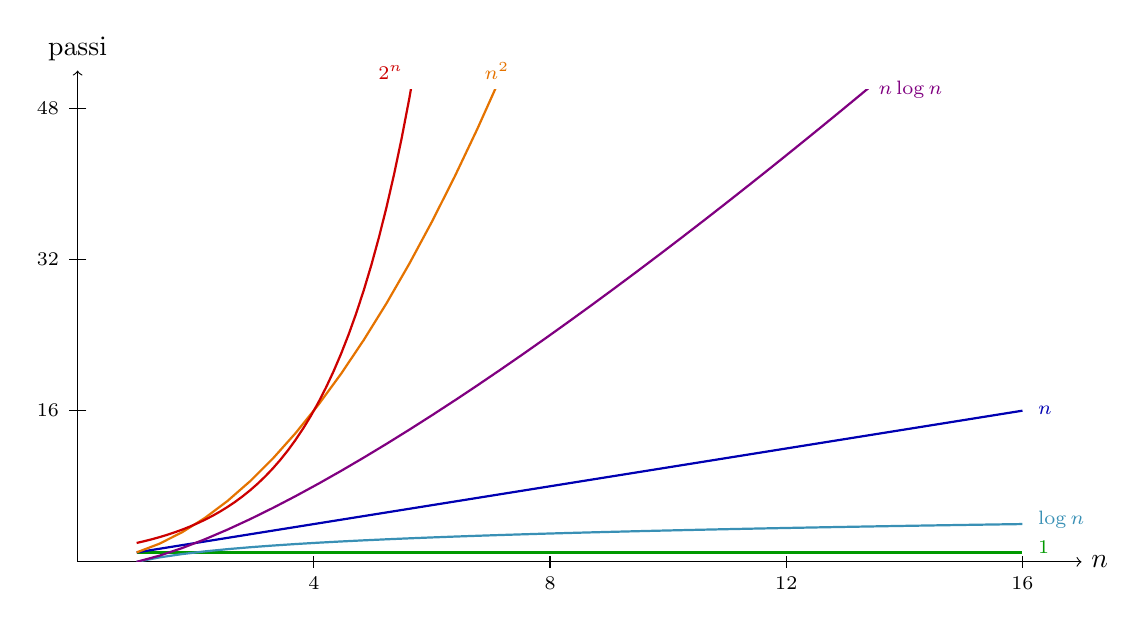
\begin{tikzpicture}[x=0.75cm,y=0.12cm]
  \draw[->] (0,0) -- (17,0) node[right] {$n$};
  \draw[->] (0,0) -- (0,52) node[above] {passi};
  \foreach \x in {4,8,12,16} \draw (\x,0.6) -- (\x,-0.6) node[below,font=\scriptsize] {\x};
  \foreach \y in {16,32,48} \draw (0.15,\y) -- (-0.15,\y) node[left,font=\scriptsize] {\y};
  \begin{scope}
    \clip (0,0) rectangle (17,50);
    \draw[thick,green!60!black] plot[domain=1:16] (\x,1);
    \draw[thick,cyan!70!black] plot[domain=1:16,samples=40] (\x,{ln(\x)/ln(2)});
    \draw[thick,blue!70!black] plot[domain=1:16] (\x,\x);
    \draw[thick,violet] plot[domain=1:16,samples=40] (\x,{\x*ln(\x)/ln(2)});
    \draw[thick,orange!90!black] plot[domain=1:16,samples=40] (\x,{\x*\x});
    \draw[thick,red!80!black] plot[domain=1:6,samples=40] (\x,{2^\x});
  \end{scope}
  \node[font=\scriptsize,text=green!60!black,anchor=west] at (16.1,1.5) {$1$};
  \node[font=\scriptsize,text=cyan!70!black,anchor=west] at (16.1,4.5) {$\log n$};
  \node[font=\scriptsize,text=blue!70!black,anchor=west] at (16.1,16) {$n$};
  \node[font=\scriptsize,text=violet,anchor=west] at (13.4,50) {$n\log n$};
  \node[font=\scriptsize,text=orange!90!black,anchor=south] at (7.1,50) {$n^2$};
  \node[font=\scriptsize,text=red!80!black,anchor=south] at (5.3,50) {$2^n$};
\end{tikzpicture}
\end{center}

\needspace{5cm}
\textbf{Dimezzare: perché $\log n$ passi.} Ricerca in un array ordinato di 16
elementi: a ogni passo resta metà dello spazio. $16 \to 8 \to 4 \to 2 \to 1$: 4 passi,
e $2^4 = 16$.
\begin{center}
\begin{tikzpicture}
  \foreach \riga/\da/\a [count=\r] in {0/0/15,1/8/15,2/8/11,3/10/11,4/10/10} {
    \foreach \i in {0,...,15} {
      \pgfmathsetmacro{\attivo}{(\i>=\da && \i<=\a) ? 1 : 0}
      \ifdim\attivo pt>0.5pt
        \node[cellina,minimum width=0.55cm,minimum height=0.5cm,fill=heapcol,font=\tiny] at (\i*0.55,-\riga*0.65) {};
      \else
        \node[cellina,minimum width=0.55cm,minimum height=0.5cm,fill=black!10!sfondo,draw=black!30,font=\tiny] at (\i*0.55,-\riga*0.65) {};
      \fi
    }
    \node[etichetta,anchor=east] at (-0.5,-\riga*0.65) {passo \riga};
  }
  \node[etichetta,anchor=west,text width=4.2cm] at (9.2,-1.3) {in arancione la parte in cui il valore può ancora trovarsi: si dimezza a ogni confronto};
\end{tikzpicture}
\end{center}

\needspace{6cm}
\textbf{Divide et impera: perché $N \log N$.} Ricorrenza $C_N = 2C_{N/2} + N$ con
$N = 8$. Ogni livello divide i pezzi a metà; a ogni livello il lavoro di
``ricombinazione'' tocca in tutto $N$ elementi. I livelli sono $\log_2 8 = 3$.
\begin{center}
\begin{tikzpicture}
  \node[cella,fill=stackcol,minimum width=6.4cm] (l0) at (0,0) {8};
  \foreach \i in {0,1} \node[cella,fill=stackcol,minimum width=3.1cm] (l1\i) at (-1.65+\i*3.3,-1) {4};
  \foreach \i in {0,...,3} \node[cella,fill=stackcol,minimum width=1.5cm] (l2\i) at (-2.4+\i*1.6,-2) {2};
  \foreach \i in {0,...,7} \node[cella,fill=stackcol,minimum width=0.7cm] (l3\i) at (-2.8+\i*0.8,-3) {1};
  \foreach \y/\t in {0/lavoro 8,-1/lavoro 4+4 = 8,-2/lavoro 2+2+2+2 = 8,-3/casi base} \node[etichetta,anchor=west] at (3.6,\y) {\t};
  \draw[decorate,decoration={brace,amplitude=5pt}] (-3.9,-3) -- (-3.9,0) node[midway,left=6pt,etichetta,text width=2cm,align=right] {$\log_2 8 = 3$ livelli};
  \node[font=\small,anchor=north] at (0,-3.6) {totale: $3$ livelli $\times$ $8$ = $N \log N$};
\end{tikzpicture}
\end{center}

% ---------------------------------------------------------------------
\section{Pattern di Codice di Laboratorio}
% ---------------------------------------------------------------------

Il ``contatore di passi'': una variabile globale \cc|passi| che ogni funzione
incrementa a ogni operazione elementare. Il \cc|main| esegue cinque funzioni di
complessità diversa per $n$ = 10, 100, 1000, 10\,000 e stampa i passi. Le funzioni
sono passate a \cc|conta| come \textbf{puntatori a funzione} (Modulo 3).

\codice{codice/m06/pattern.cpp}
\uscita{codice/m06/output/pattern.txt}

\textbf{Cosa osservare:} leggi la tabella \emph{per colonne}. Quando $n$ si
moltiplica per 10, la colonna $O(1)$ resta ferma, $O(\log n)$ cresce di 3--4,
$O(n)$ si moltiplica per 10, $O(n^2)$ per 100. Questo è tutto quello che dice la
notazione O-grande.

% ---------------------------------------------------------------------
\section{Tips \& Trappole da Esame}
% ---------------------------------------------------------------------

\begin{trappola}[: le costanti non contano]
$O(2n)$, $O(n/2)$ e $O(n + 100)$ si scrivono tutti $O(n)$. Scrivere $O(2n)$ in un
quiz non è sbagliato in senso stretto, ma mostra di non aver capito il punto.
\end{trappola}

\begin{trappola}[: annidati contro in sequenza]
Due cicli da $n$ \textbf{uno dentro l'altro} fanno $O(n^2)$; \textbf{uno dopo
l'altro} fanno $O(n) + O(n) = O(n)$. Guarda le graffe, non il numero di \cc|for|.
\end{trappola}

\begin{trappola}[: il ciclo interno non dipende sempre da n]
\cc|for (i = 0; i < n; i++) for (j = 0; j < 5; j++)| è $O(n)$: il ciclo interno fa
sempre 5 giri, è una costante. Conta i giri, non i cicli.
\end{trappola}

\begin{trappola}[: O-grande è un limite, non una misura esatta]
``L'algoritmo è $O(n^2)$'' è vero anche per un algoritmo lineare. Se il quiz chiede
quale affermazione è \emph{vera}, $O$ più grandi del necessario sono vere; se chiede
la complessità, dai la più stretta.
\end{trappola}

\begin{trappola}[: anche le chiamate costano]
Un ciclo da $n$ giri che chiama una funzione $O(n)$ a ogni giro è $O(n^2)$, anche se
vedi un solo \cc|for|. Ad esempio: chiamare una ricerca lineare dentro un ciclo.
\end{trappola}

\begin{consiglio}[: il metodo del raddoppio]
Se non sei sicuro della complessità di un pezzo di codice, aggiungi un contatore e
prova con $n$ e $2n$. Passi uguali: $O(1)$. Più uno: $O(\log n)$. Doppi: $O(n)$.
Quadruplicati: $O(n^2)$. Otto volte: $O(n^3)$.
\end{consiglio}

% ---------------------------------------------------------------------
\section{Quiz a Crocette (Prova Scritta)}
% ---------------------------------------------------------------------

\begin{quiz}{Qual è la complessità di \texttt{for (i = 0; i < n; i += 3) somma += i;}?}
  \item $O(1)$
  \item $O(\log n)$
  \item $O(n)$
  \item $O(n/3)$, diversa da $O(n)$
\end{quiz}

\begin{quiz}{Qual è la complessità di \texttt{for (i = 1; i < n; i *= 2) cont++;}?}
  \item $O(n)$
  \item $O(\log n)$
  \item $O(n^2)$
  \item $O(2^n)$
\end{quiz}

\begin{quiz}{Due cicli \texttt{for} da $n$ giri ciascuno, scritti uno \textbf{dopo} l'altro (non annidati). Complessità totale?}
  \item $O(n)$
  \item $O(n^2)$
  \item $O(2n^2)$
  \item $O(\log n)$
\end{quiz}

\begin{quiz}{$T(n) = 4n^3 + 100n^2 + 7$. Quale affermazione è \textbf{vera}?}
  \item $T(n) = O(n^2)$
  \item $T(n) = O(n^3)$
  \item $T(n) = O(100n^2)$
  \item $T(n) = O(7)$
\end{quiz}

\begin{quiz}{Se un algoritmo è $O(n^2)$, quale affermazione è sicuramente vera?}
  \item è anche $O(n^3)$
  \item è anche $O(n)$
  \item è anche $\Omega(n^2)$
  \item impiega esattamente $n^2$ passi
\end{quiz}

\begin{quiz}{Cosa significa $f(n) = \Theta(g(n))$?}
  \item $f$ cresce al più come $g$
  \item $f$ cresce almeno come $g$
  \item $f$ cresce esattamente come $g$: è sia $O(g)$ sia $\Omega(g)$
  \item $f$ e $g$ sono la stessa funzione
\end{quiz}

\begin{quiz}{Quale ordine di crescita è corretto, dal più lento al più veloce?}
  \item $\log n,\ n,\ n\log n,\ n^2,\ 2^n$
  \item $n,\ \log n,\ n^2,\ n\log n,\ 2^n$
  \item $\log n,\ n\log n,\ n,\ 2^n,\ n^2$
  \item $1,\ n,\ \log n,\ n^2,\ n\log n$
\end{quiz}

\begin{quiz}{La ricorrenza $C_N = 2C_{N/2} + N$ (divido a metà, risolvo le due metà, scorro tutto) ha soluzione:}
  \item $O(N)$
  \item $O(\log N)$
  \item $O(N \log N)$
  \item $O(N^2)$
\end{quiz}

\begin{quiz}{Un algoritmo di ordinamento per confronti ha complessità $O(n \log n)$. Sapendo che il problema è $\Omega(n \log n)$, l'algoritmo è:}
  \item ottimo
  \item migliorabile fino a $O(n)$
  \item esponenziale
  \item non si può dire nulla
\end{quiz}

\begin{quiz}{In una ricerca lineare su un array di $n$ elementi, il caso peggiore è:}
  \item l'elemento cercato è il primo
  \item l'elemento cercato è a metà
  \item l'elemento è l'ultimo o non è presente
  \item l'array è vuoto
\end{quiz}

\begin{quiz}{Qual è la complessità in \textbf{spazio} della potenza ricorsiva \texttt{pot(x, n) = x * pot(x, n-1)}?}
  \item $O(1)$, perché non usa array
  \item $O(n)$, perché le $n$ chiamate sono contemporaneamente nello stack
  \item $O(\log n)$
  \item $O(n^2)$
\end{quiz}

\begin{soluzione}[: risposte commentate]
\begin{enumerate}[label=\textbf{\arabic*.}]
  \item \textbf{C}. Circa $n/3$ giri: la costante $1/3$ si ignora. La D è il
        distrattore: $O(n/3)$ e $O(n)$ sono la stessa cosa.
  \item \textbf{B}. \cc|i| raddoppia: si arriva a $n$ in circa $\log_2 n$ passi.
  \item \textbf{A}. In sequenza si sommano: $n + n = 2n$, cioè $O(n)$.
  \item \textbf{B}. Vince il termine $n^3$. La C è uguale ad $O(n^2)$ ed è falsa.
  \item \textbf{A}. O-grande è un limite superiore: un limite più alto è ancora
        valido. Le altre non sono garantite.
  \item \textbf{C}. Definizione di $\Theta$.
  \item \textbf{A}.
  \item \textbf{C}. È la ricorrenza del MergeSort: $\log N$ livelli da $N$ di lavoro.
  \item \textbf{A}. Limite superiore dell'algoritmo e limite inferiore del problema
        coincidono.
  \item \textbf{C}. Servono $n$ confronti.
  \item \textbf{B}. Ogni chiamata occupa un record di attivazione finché le
        successive non terminano.
\end{enumerate}
\end{soluzione}

% ---------------------------------------------------------------------
\section{Laboratorio a Step (Simulazione d'Esame)}
% ---------------------------------------------------------------------

\begin{traccia}[: segmento di somma massima (dalle slide)]
Dato un array \cc|S| di $n$ interi (positivi e negativi, almeno uno positivo), un
\emph{segmento} è una sequenza di elementi \textbf{consecutivi} \cc|S[i..j]|. Si vuole
trovare il segmento con la \textbf{somma massima}; a parità di somma si preferisce il
segmento più corto. Si scriveranno tre algoritmi via via più efficienti e se ne
misurerà il costo.
\end{traccia}

\begin{step}{il contatore}
Dichiara una variabile globale \cc|long long passi| che ogni algoritmo incrementerà
a ogni somma di un elemento. Azzerala prima di ogni misura.\\[0.3em]
\textbf{Concetto nuovo:} misurare la complessità sperimentalmente.
\end{step}

\begin{step}{la soluzione ingenua}
Scrivi \cc|int sommaMassima1(const int S[], int n)|: per ogni coppia \cc|(i, j)| con
\cc|i <= j| calcola da capo la somma di \cc|S[i..j]| con un terzo ciclo. Prima di
eseguirla, prevedi la complessità.\\[0.3em]
\textbf{Concetto nuovo:} tre cicli annidati, $O(n^3)$.
\end{step}

\begin{step}{non ricalcolare}
Scrivi \cc|sommaMassima2|: osserva che la somma di \cc|S[i..j]| è la somma di
\cc|S[i..j-1]| più \cc|S[j]|, quindi non serve il terzo ciclo.\\[0.3em]
\textbf{Concetto nuovo:} riusare risultati già calcolati, da $O(n^3)$ a $O(n^2)$.
\end{step}

\begin{step}{una sola passata}
Scrivi \cc|int sommaMassima3(const int S[], int n, int& inizio, int& fine)|, che
scorre l'array \textbf{una volta} tenendo una somma ``in corso'': se diventa negativa,
la azzera e fa ripartire il segmento dall'elemento successivo (una somma negativa
può solo peggiorare quello che viene dopo). Restituisci anche gli estremi del
segmento, preferendo il più corto a parità di somma.\\[0.3em]
\textbf{Concetto nuovo:} un'idea migliore batte un computer più veloce, $O(n)$.
\end{step}

\begin{step}{il confronto}
Con \cc|srand(111222333)| genera array casuali di 10, 100 e 1000 elementi (valori
tra $-10$ e $10$) e stampa una tabella con i passi dei tre algoritmi, verificando che
diano tutti lo stesso risultato.\\[0.3em]
\textbf{Concetto nuovo:} leggere la crescita in una tabella.
\end{step}

\subsection*{Soluzione completa}
\codice{codice/m06/lab.cpp}
\uscita{codice/m06/output/lab.txt}

\begin{consiglio}[: cosa notare nella soluzione]
\begin{itemize}
  \item Da $n = 100$ a $n = 1000$ (dati $\times 10$): la versione cubica passa da
        171\,700 a 167 milioni di passi ($\times 1000$), la quadratica da 5050 a
        500\,500 ($\times 100$), la lineare da 100 a 1000 ($\times 10$).
  \item I numeri della quadratica sono esattamente $\frac{n(n+1)}{2}$ (la somma di
        Gauss), quelli della cubica circa $\frac{n^3}{6}$: le costanti cambiano, la
        crescita no.
  \item Sull'esempio piccolo il segmento migliore è \texttt{S[2..5]} =
        $3 + 5 - 2 + 4 = 10$.
\end{itemize}
\end{consiglio}

% ---------------------------------------------------------------------
\section{Domande e Risposte Modello per l'Orale}
% ---------------------------------------------------------------------

\begin{orale}[D1. Come si misura la complessità di un algoritmo?]
La si esprime in funzione della dimensione $n$ dell'input, contando il numero di
operazioni elementari eseguite (complessità temporale, nel modello RAM ogni
operazione costa 1) o il numero di celle di memoria aggiuntive (complessità
spaziale). Il costo di una sequenza è la somma dei costi; quello di un
\cc|if| è il costo della guardia più il maggiore dei due rami; quello di un ciclo è
la somma dei costi di tutte le iterazioni. Di solito si considera il caso peggiore e
si studia il comportamento asintotico, cioè come cresce il costo per $n$ grande,
ignorando costanti e termini di ordine inferiore.
\end{orale}

\begin{orale}[D2. Cosa significa O-grande?]
$f(n) = O(g(n))$ se esistono una costante $c > 0$ e un $n_0$ tali che
$f(n) \le c \cdot g(n)$ per ogni $n > n_0$. In parole: da un certo punto in poi $f$
non cresce più velocemente di $g$, a meno di una costante. È un limite superiore
asintotico; non è unico, perché anche ogni funzione più grande lo è, e per questo si
indica il più piccolo noto.
\end{orale}

\begin{orale}[D3. Differenza tra O, Omega e Theta?]
$O$ è un limite superiore: $f$ cresce al più come $g$. $\Omega$ è un limite inferiore:
$f$ cresce almeno come $g$, cioè $f(n) \ge c \cdot g(n)$ da un certo $n$ in poi.
$\Theta$ indica che valgono entrambi, quindi $f$ cresce esattamente come $g$. Per un
problema, se un algoritmo ha costo $O(f(n))$ e si dimostra che il problema richiede
$\Omega(f(n))$, l'algoritmo è ottimo e la complessità del problema è $\Theta(f(n))$:
è il caso dell'ordinamento per confronti con $n \log n$.
\end{orale}

\begin{orale}[D4. Quali sono le principali classi di complessità?]
In ordine crescente: costante $O(1)$, logaritmica $O(\log n)$, lineare $O(n)$,
$O(n \log n)$, polinomiale (quadratica $O(n^2)$, cubica $O(n^3)$, \ldots) ed
esponenziale $O(c^n)$. Un ciclo con incremento costante è lineare, uno che
moltiplica o divide per una costante è logaritmico, cicli annidati moltiplicano le
complessità. Gli algoritmi esponenziali sono impraticabili già per input piccoli.
\end{orale}

\begin{orale}[D5. Come si analizza un algoritmo ricorsivo?]
Si scrive una relazione di ricorrenza che esprime il costo per $n$ in funzione del
costo sui sottoproblemi più piccoli più il lavoro della singola chiamata. Alcune
ricorrenze fondamentali: $C_N = C_{N-1} + N$ dà $O(N^2)$; $C_N = C_{N/2} + 1$ dà
$O(\log N)$, come la ricerca binaria; $C_N = 2C_{N/2} + N$ dà $O(N \log N)$, tipica
del divide et impera come il MergeSort. Ad esempio la potenza $x^n$ calcolata come
$x \cdot x^{n-1}$ costa $O(n)$, mentre calcolata dimezzando l'esponente costa
$O(\log n)$. Nella ricorsione va considerato anche lo spazio: ogni chiamata attiva
occupa un record nello stack.
\end{orale}

% ---------------------------------------------------------------------
\section{Esercizi al PC}
% ---------------------------------------------------------------------

In ogni esercizio: \textbf{prima} scrivi su un foglio la complessità che ti
aspetti, \textbf{poi} aggiungi un contatore al codice e controlla con i numeri.

\begin{esercizio}{Un passo sì e uno no}{facile}
Conta i giri di \cc|for (i = 0; i < n; i += 2)| per $n$ = 10, 100, 1000, 10\,000 e
stampa anche \cc|passi / n|. Cosa noti nel rapporto? Che complessità è?
\end{esercizio}

\begin{esercizio}{Quadrato e triangolo}{facile}
Conta i giri di due cicli annidati completi (\cc|j| da 0 a $n$) e di due cicli ``a
triangolo'' (\cc|j| da \cc|i+1| a $n$). Stampa i rapporti con $n^2$. Hanno la stessa
complessità?
\end{esercizio}

\begin{esercizio}{Raddoppiare}{facile}
Conta i giri di \cc|for (i = 1; i < n; i *= 2)| per $n$ = 1, 10, 100, \ldots,
1\,000\,000. Di quanto crescono i passi quando $n$ si moltiplica per 10?
\end{esercizio}

\begin{esercizio}{Vince il più pesante}{facile}
Metti in sequenza un ciclo da $n$ giri e due cicli annidati da $n$. Stampa i passi
dei due blocchi e la percentuale di lavoro del secondo per $n$ = 10, 100, 1000.
\end{esercizio}

\begin{esercizio}{I tre casi della ricerca lineare}{medio}
Su un array di 1000 elementi, conta i confronti della ricerca lineare nel caso
migliore, nel caso peggiore (ultimo elemento e assente) e nel caso medio (media
cercando, uno alla volta, tutti gli elementi presenti).
\end{esercizio}

\begin{esercizio}{L'esempio delle slide}{medio}
Implementa la funzione \cc|func(n)| delle slide (ciclo esterno da $n/2$ a $n$, due
cicli interni che raddoppiano) e verifica che \cc|count| sia esattamente
$(n/2 + 1) \cdot L \cdot L$, dove $L$ è il numero di giri di un ciclo che raddoppia
fino a $n$. Che complessità ne deduci?
\end{esercizio}

\begin{esercizio}{Potenza lenta e veloce}{medio}
Implementa le due versioni ricorsive della potenza delle slide e conta le
moltiplicazioni per $2^{10}$, $2^{30}$, $2^{62}$ (usa \cc|long long|).
\end{esercizio}

\begin{esercizio}{Numeri primi}{medio}
Scrivi due test di primalità: uno che prova tutti i divisori da 2 a $n-1$ e uno che si
ferma quando \cc|d * d > n|. Conta le divisioni sui numeri primi 97, 9973 e 999\,983 e
spiega perché basta arrivare alla radice quadrata.
\end{esercizio}

\begin{esercizio}{Lineare contro binaria}{difficile}
Su array ordinati di $10^3$, $10^5$ e $10^6$ elementi (allocati con \cc|new|), conta
i confronti della ricerca lineare e della ricerca binaria cercando un valore assente.
\end{esercizio}

\begin{esercizio}{Fibonacci}{difficile}
Scrivi Fibonacci ricorsivo ``ingenuo'' e iterativo e confronta il numero di chiamate
ricorsive con il numero di giri del ciclo per $n$ = 10, 15, \ldots, 35. Di quanto si
moltiplicano le chiamate a ogni $+5$?
\end{esercizio}

\subsection*{Soluzioni}
Le soluzioni commentate, con il codice e l'output reale, sono nel PDF separato
\textbf{Soluzioni} (\texttt{soluzioni-light.pdf} / \texttt{soluzioni-dark.pdf}),
allo stesso numero di esercizio. Il codice è anche in \texttt{codice/m06/}.
